\documentclass[12pt]{article}

\usepackage[margin=1in]{geometry} % sets margins
\usepackage{graphicx}             % import figures
\usepackage{subcaption}           % Subsections
\usepackage{pgfplotstable}        % Generates tables from .csv files
\usepackage{siunitx}
\usepackage{floatrow}

\newfloatcommand{capbtabbox}{table}[][\FBwidth]

\pgfplotsset{compat=newest}
\usepgfplotslibrary{units}

\sisetup{
  round-mode      = places,
  round-precision = 2,
}

\title{Testing Scheduling Algorithms}
\author{
  Michael Nutt
  \and
  Nathan Burgess
  \and
  Jeremiah Dickens
}
\date{}

\begin{document}

\maketitle
\pagenumbering{gobble}
\newpage
\pagenumbering{roman}
\tableofcontents
\newpage
\pagenumbering{arabic}

\section{Introduction}

  \subsection{The Problem}

  Operating Systems have the complex task of scheduling processes to maximize efficiency while following rules for priority. For this assignment we were tasked with implementing a scheduler that took 200 processes that were created randomly with cycle counts between $10*10^{6}$ and $50*10^{12}$ cycles and sizes ranging from .25 MB to 8 GB. To simplify the simulation, for the first three scenarios it is assumed that all 200 processes came in simultaneously and can be sorted in any way we want, and that there is no preemption. This second requirement limited our options for possible algorithms used to solve the problem, we decided to test First-In-First-Out, Shortest Job First, and one we created that is similar to Shortest Job First, titled Modified Shortest Job First.

  \subsection{The Environment}

  For our solution the target computer has five processor cores that had a variety of scenarios applied to them. For the first program it was assumed all things were equal. For easier comparison the cores were set to 4 GHz and memory was assumed to be sufficient for any process coming in. The second scenario had variable memory sizes, the third scenario had variable processor speeds. The fourth scenario was assumed all things equal again, with the caveat that the processes entered in order, preventing pre-sorting of the processes to optimize order.

  \subsection{Algorithms Used}
    \paragraph{First-In-First-Out}

    First In First Out is implemented with no sorting, the first process in the list runs, followed by the next and so on.

    \paragraph{Shortest Job First}

    Shortest Job First is implemented by first sorting the process list in order of cycle count, then running through the list from first to last.

    \paragraph{Modified Shortest Job First}

    Modified Shortest Job First takes the main principle of Shortest Job First, sorting the processes by cycle count. Assignment goes by placing the longest job in the first processor, then shortest jobs in the remaining four. When the longest job completes that processor is assigned a short job, then the next available processor takes the next longest job. The processors rotate in this manner until all processes are completed.

  \subsection{Performance Measurement}

  For this experiment we are focused on the total running time to measure which algorithm is better than others. We chose this measurement based on the assumptions that all processes are arriving at the same time and that there is no preemption of processes that are currently running.

\newpage
\section{Experimental Results}

For the following experiments we generated 50 sets of 200 processes for the processors to run, each experiment using the same set of 50 processes.

  \subsection{All Things Equal}

  This scenario had equal clock speeds across the board and the assumption that each processor would have enough memory to run the processes. From a theoretical standpoint, First In First Out and Shortest Job First should have a similar average running time as the processors are running at equal processing speeds.

  \begin{figure}[h!]\CenterFloatBoxes
  \begin{floatrow}
    \ffigbox[\FBwidth]
    {
      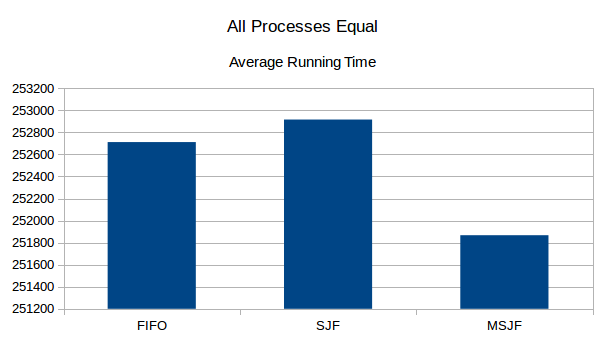
\includegraphics[width=\linewidth]{Data/EqualProcessorSpeeds}
    }
    {\caption{Average running time of equal processors}}
    \killfloatstyle\ttabbox[\Xhsize]
    {
      \begin{tabular}{c|c|c}
        \textbf{FIFO} & \textbf{SJF} & \textbf{MSJF}\\
        \hline
        252,712 & 252,916 & 251,867\\
      \end{tabular}
    }
    {\caption{Average running time of equal processors in seconds}}
  \end{floatrow}
  \end{figure}

  As can be seen in the figures FIFO and SJF had average running times that were within 200 seconds of each other, while MSJF was faster by almost 1,000 seconds. This can be explained by the method of tackling some of the larger jobs first to ensure toward the end of the list longer jobs aren't stacked on the processors.

  \subsection{Variable Memory Sizes}

  This scenario had all processors equal in clock speed but with variable memory capacity sizes, with processor $P_A$ and $P_B$ at 2 GB, $P_C$ and $P_D$ at 4 GB and $P_E$ at 8 GB. In a theoretical scenario this could affect the downtime of individual processors, as a realistic model of processes could see lower cycle count processes using less memory and higher cycle processes using more, so a Shortest Job First approach could mean that lower storage capacity processors would be underutilized as the lower memory processes completed, with eventually just one processor running as jobs exceeded the 2 and 4 GB size limits.

  \begin{figure}[h!]\CenterFloatBoxes
  \begin{floatrow}
    \ffigbox[\FBwidth]
    {
      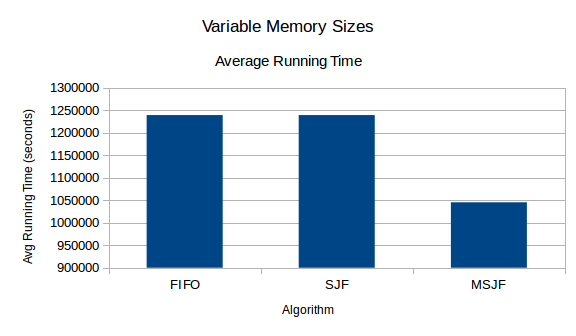
\includegraphics[width=\linewidth]{Data/VariableMemorySizesAVG}
    }
    {\caption{Average running time of variable memory per algorithm}}
    \killfloatstyle\ttabbox[\Xhsize]
    {
      \begin{tabular}{c|c|c}
        \textbf{FIFO} & \textbf{SJF} & \textbf{MSJF}\\
        \hline
        1,239,737 & 1,239,737 & 1,045,704\\
      \end{tabular}
    }
    {\caption{Average running time of variable memory in seconds}}
  \end{floatrow}
  \end{figure}

  As shown in Figure 1 and Table 1, in this scenario with our randomly generated processes the First In First Out and Shortest Time First algorithms produced the same total running time. The Modified Shortest Job First had the shortest run time as it balanced the load for longer processes and shorter processes, helping to prevent starvation of longer processes.

  \newpage
  \subsection{Variable Processor Speeds}

  This scenario had the processors running at different clock speeds with memory capacities equal, with the clock speeds for $P_A$ and $P_B$ at 2 GHz, $P_C$ and $P_D$ at 3 GHz and $P_E$ at 4 GHz. This presented situations where the scheduler could more carefully analyze the clock cycles needed to match it with an appropriate speed processor for optimal performance. Because of this the Modified Shortest Job First algorithm was modified further for this scenario, instead placing all the shortest jobs on $P_A$ and $P_B$, the longest jobs on $P_E$ and alternating between a long and short job on $P_C$ and $P_D$.

  \begin{figure}[h!]\CenterFloatBoxes
  \begin{floatrow}
    \ffigbox[\FBwidth]
    {
      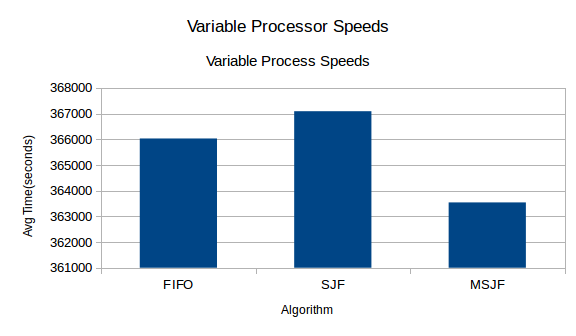
\includegraphics[width=\linewidth]{Data/VariableProcessorSpeedsAVG}
    }
    {\caption{Average running time of variable memory per algorithm}}
    \killfloatstyle\ttabbox[\Xhsize]
    {
      \begin{tabular}{c|c|c}
        \textbf{FIFO} & \textbf{SJF} & \textbf{MSJF}\\
        \hline
        366,032 & 367,093 & 363,542\\
      \end{tabular}
    }
    {\caption{Average running time of variable memory in seconds}}
  \end{floatrow}
  \end{figure}

  As can be seen in the Figure 2 and Table 2, with the variable clock speeds associated with each processor, Shortest Job First performed worse than First-In-First-Out. This is due to all the shortest processes going through first on the different speed levels, then the longer processes getting bottle necked on the slower 2 GHz $P_A$ and $P_B$ processors, increasing the total time required to complete all processes. It is also shown that the Modified Shortest Job First performed the best, as it took into consideration the different speeds to ensure proper load balancing of the processors.

  \subsection{All Things Equal, Processes Arrive in Order}

  For this scenario we were assuming that the processes were arriving in order, limiting our approach to assigning them to the processors since we are also assuming no preemption on the processors. For this scenario the method we used was First In First Out, which yielded an average time of 252,712 seconds for processing.

\section{Conclusion}

After running the trials for each scenario we found that the First In First Out method was often equal to or faster than the Shortest Job First method, while our Modified Shortest Job First generated the shortest running time. These numbers do rely on the fact that we know the exact running speed of all 200 processes and that we are able to order them all the same. In a real world scenario where the processes are arriving at random times a better solution could be created by creating process priorities and allowing the scheduler to preempt processes to ensure equal time on the processor per priority level. With preemption the final scenario could have been adapted with a Modified Shortest Time Remaining that alternates with longer jobs added in to prevent starvation, and only allowing jobs to run a set amount of cycles before preempting for the next in line. 

\newpage
\begin{appendix}
  \listoffigures
  \listoftables
\end{appendix}

\end{document}
